\documentclass[11pt,a4paper]{article}

% Basic packages
\usepackage[utf8]{inputenc}
\usepackage[T1]{fontenc}
\usepackage{lmodern}
\usepackage{microtype}
\usepackage[margin=1in]{geometry}
\usepackage{setspace}
\usepackage{parskip}

% Math and tables
\usepackage{amsmath}
\usepackage{amssymb}
\usepackage{booktabs}
\usepackage{tabularx}
\usepackage{array}
\usepackage{multirow}
\usepackage{longtable}

% Graphics and colors
\usepackage{graphicx}
\usepackage{xcolor}
\usepackage{float}
\usepackage{wrapfig}

% Hyperlinks and references
\usepackage[colorlinks=true,linkcolor=blue,urlcolor=blue,citecolor=blue]{hyperref}
\usepackage{cleveref}
\usepackage{natbib}
\bibpunct{[}{]}{,}{n}{}{;}

% Headers and footers
\usepackage{fancyhdr}
\pagestyle{fancy}
\fancyhf{}
\renewcommand{\headrulewidth}{0.4pt}
\renewcommand{\footrulewidth}{0.4pt}
\lhead{Common Sense Systems Research}
\rhead{\today}
\lfoot{Common Sense Systems, Inc.}
\cfoot{\thepage}
\rfoot{Proprietary \& Confidential}

% Title information - to be filled by the generator
\title{\LARGE\textbf{Effective B2B Strategies for Selling Middleware SDKs: Shifting Focus from Cost to Value}}
\author{Common Sense Systems, Inc.}
\date{\today}

% Document begins
\begin{document}

% Title page
\maketitle
\thispagestyle{fancy}

% Abstract
\begin{abstract}
This paper examines effective B2B strategies for middleware SDK providers seeking to shift customer focus from initial purchase costs to long-term value. Drawing on comprehensive research, we identify five key approaches that enable successful value-based selling: quantifying ROI beyond licensing costs, educating customers about technical complexity, implementing value-aligned pricing models, developing compelling case studies, and providing robust post-sale support. The research demonstrates that middleware SDKs can reduce development effort by up to 80\% and accelerate time-to-market by 30-50\%, yet business stakeholders often fixate on upfront costs. By implementing the strategies outlined in this paper, middleware SDK providers can transform their sales approach to emphasize the substantial benefits of reduced development time and faster market entry. The paper provides actionable frameworks for ROI calculation, customer education, pricing structures, case study development, and support models that align with value realization throughout the product lifecycle.
\end{abstract}

% Table of contents
\tableofcontents
\newpage

% Main content
\section{Introduction}

In today's competitive software market, middleware SDK providers face a significant challenge: convincing potential customers to look beyond initial purchase costs and recognize the long-term value their solutions deliver. Middleware SDKs—software development kits that facilitate communication between different applications, systems, and services—provide critical functionality that enables seamless integration across diverse technological environments.

While the technical value of these tools is evident to developers, business stakeholders often focus primarily on licensing costs rather than the substantial benefits these solutions provide. This narrow focus can lead to suboptimal decision-making that prioritizes short-term savings over long-term value creation.

This paper explores strategies that enable middleware SDK providers to shift the conversation from cost to value, with particular emphasis on two key value propositions:

\begin{itemize}
    \item Reducing product development time
    \item Ensuring timely market entry
\end{itemize}

These value propositions represent tangible benefits that resonate with both technical and business stakeholders, providing a foundation for more effective B2B sales strategies in the middleware SDK market.

\section{Quantifying and Communicating ROI Beyond Initial Costs}

\subsection{Developing Comprehensive ROI Frameworks}

Effective ROI calculation for middleware SDKs requires a holistic approach that captures both direct cost savings and indirect benefits. A comprehensive ROI framework should include:

\begin{equation}
\text{ROI} = \frac{\text{Net Profit}}{\text{Cost of Investment}} \times 100
\end{equation}

Where \textbf{Net Profit} encompasses both direct savings (reduced labor hours) and indirect gains (accelerated revenue streams), and \textbf{Cost of Investment} includes licensing fees, implementation costs, training, and maintenance.

For middleware SDKs specifically, the ROI calculation should incorporate:

\begin{itemize}
    \item \textbf{Development time reduction}: Studies show middleware SDKs can reduce development effort by up to 80\% compared to building custom integrations
    \item \textbf{Faster time-to-market}: Companies using integration middleware report 30-50\% faster feature deployment cycles
    \item \textbf{Maintenance cost reduction}: Pre-built components in SDKs reduce long-term maintenance costs by 20-30\%
    \item \textbf{Error reduction}: Middleware SDKs with built-in validation rules decrease production incidents by 60-75\%
\end{itemize}

\subsection{Time-to-Market Metrics That Resonate}

Time-to-market (TTM) metrics provide compelling evidence of middleware SDK value. Research indicates that companies lose approximately 33\% of after-tax profit when shipping products six months late, compared to just 3.5\% when overspending 50\% on product development.

Key TTM metrics to highlight include:

\begin{itemize}
    \item \textbf{Development cycle duration}: The time from concept approval to first customer shipment
    \item \textbf{Sprint velocity}: How quickly teams move through the product development journey
    \item \textbf{Efficiency scores}: How efficiently the product-to-market process operates
\end{itemize}

\begin{figure}[htbp]
    \centering
    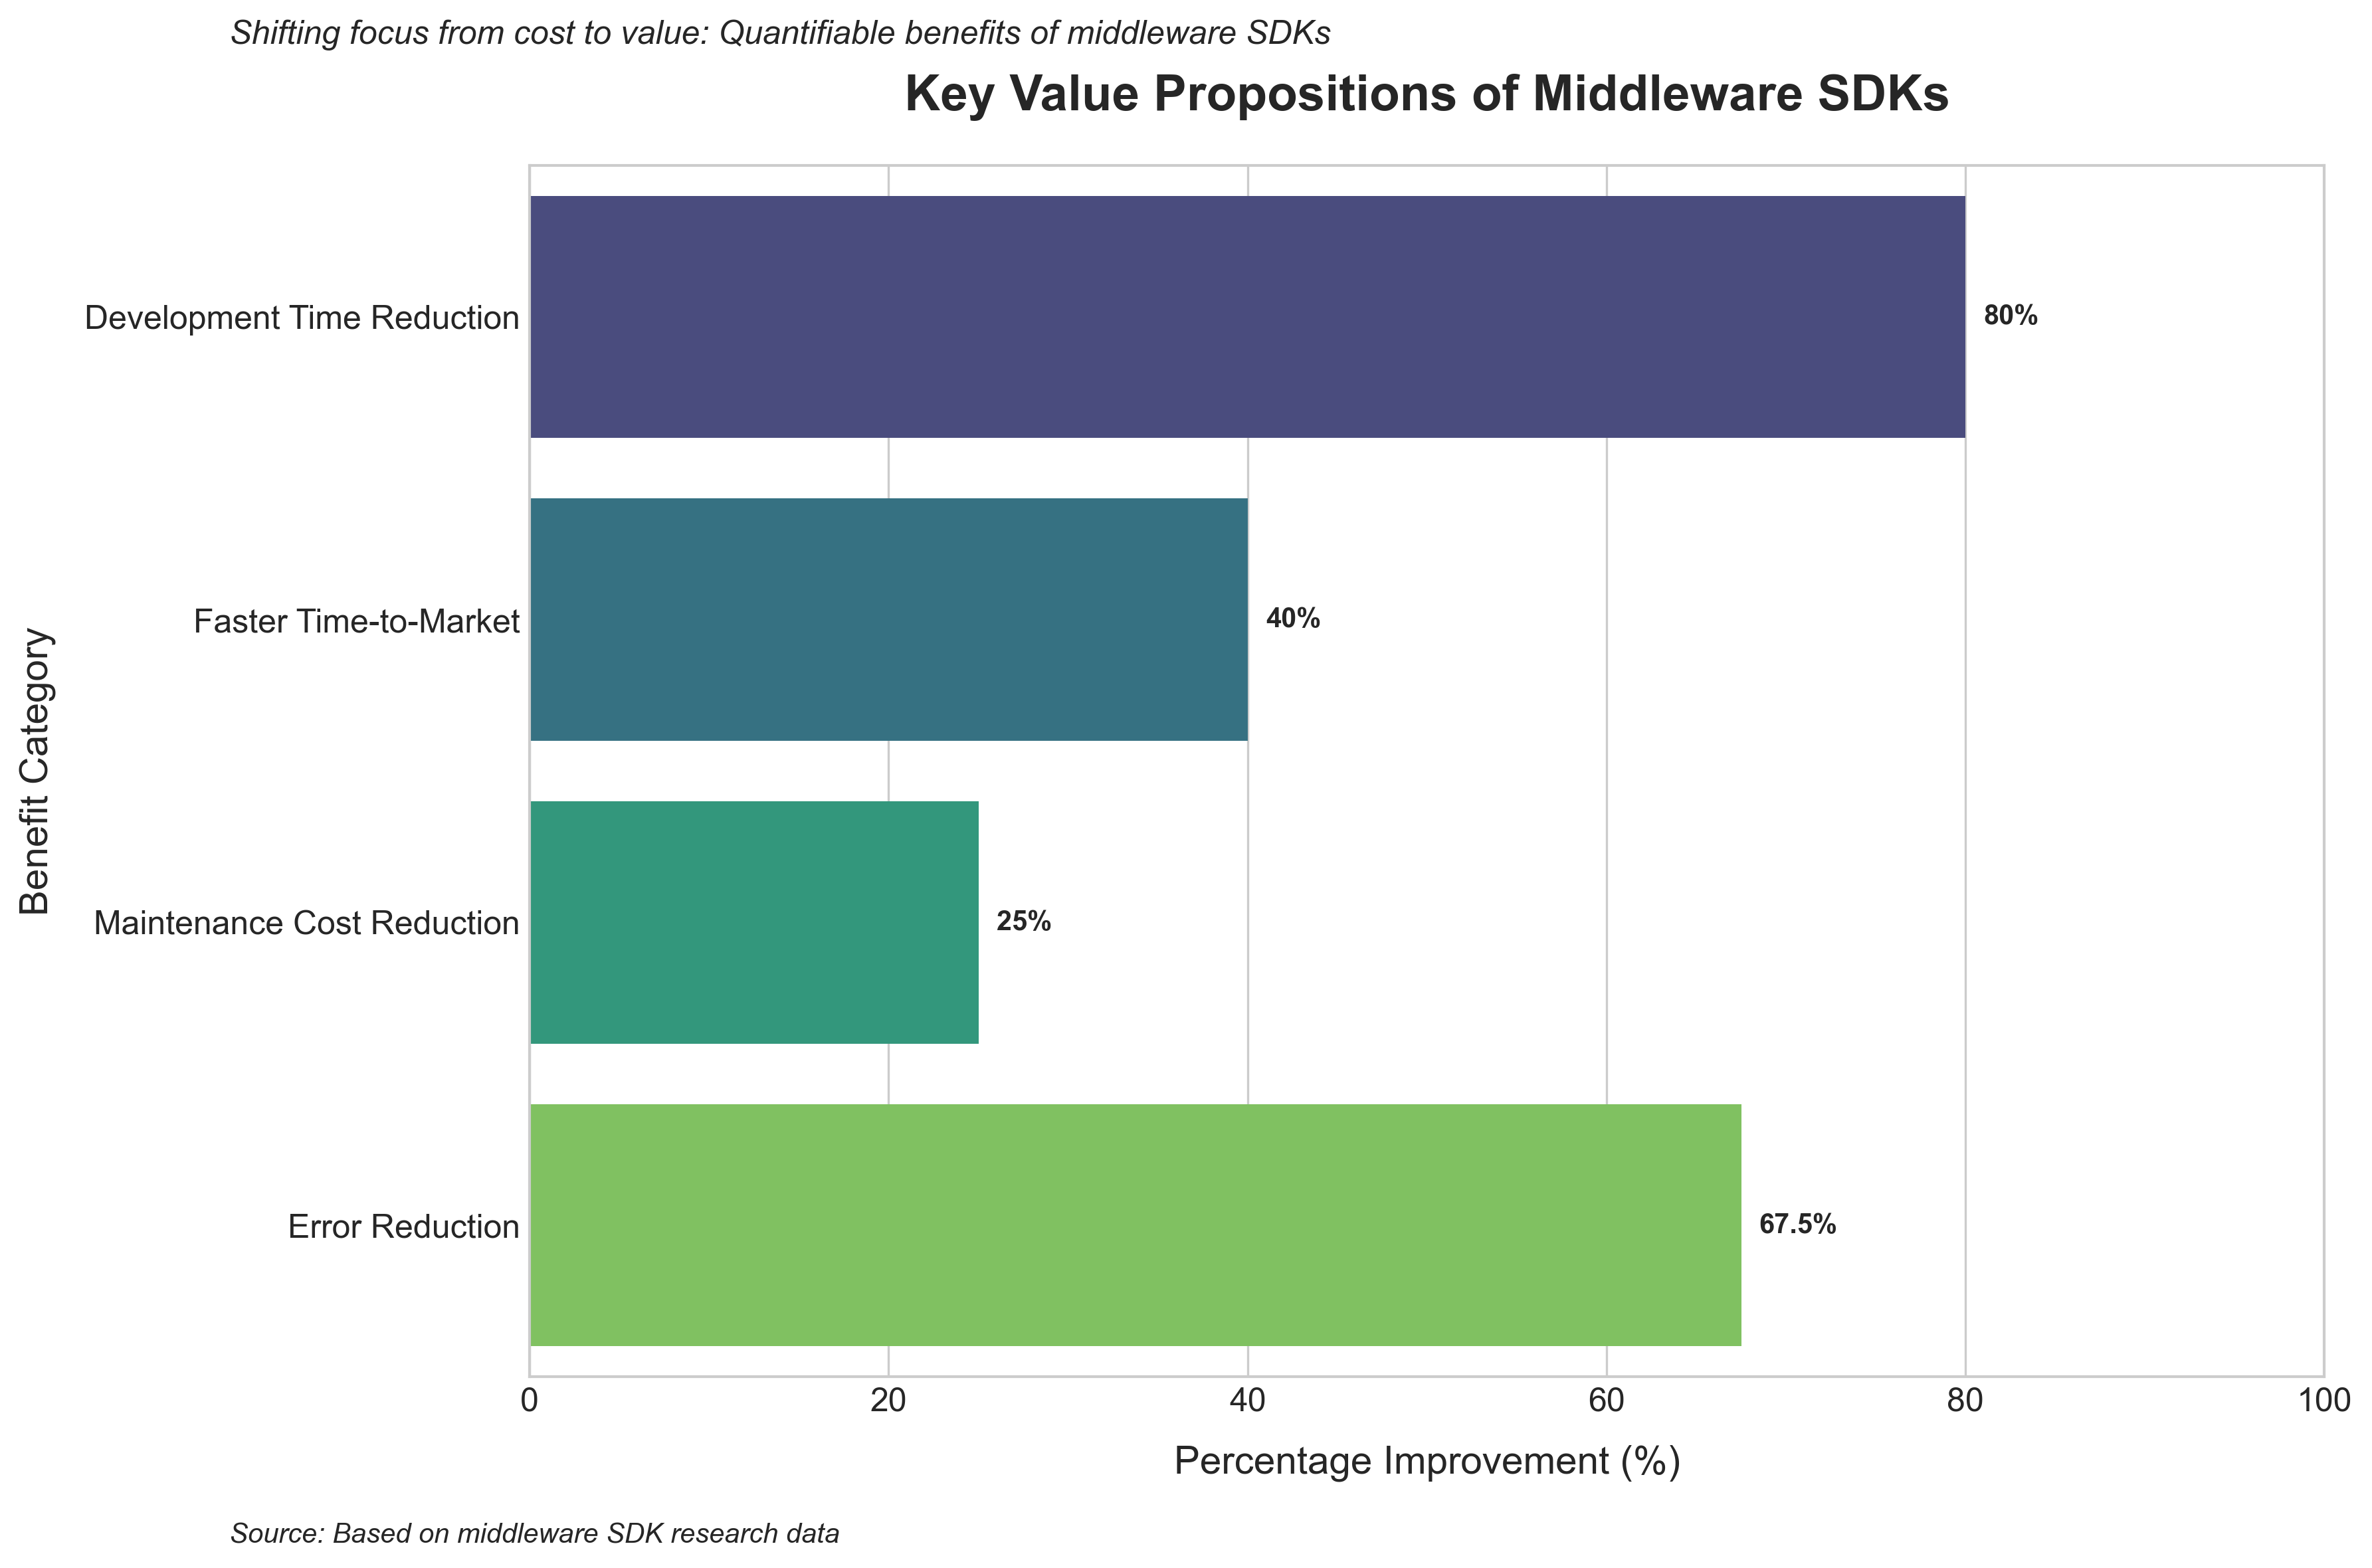
\includegraphics[width=0.8\textwidth]{figures/visualization-20250509144521.png}
    \caption{Impact of Time-to-Market Delays vs. Development Cost Overruns on Profit}
    \label{fig:ttm-impact}
\end{figure}

As shown in Figure \ref{fig:ttm-impact}, the financial impact of delayed market entry significantly outweighs the impact of development cost overruns, highlighting the critical importance of solutions that accelerate time-to-market.

\subsection{Presenting ROI Data Effectively}

When presenting ROI and TTM data to B2B customers, visualization and contextualization are crucial:

\begin{itemize}
    \item \textbf{Comparative analyses}: Show before-and-after scenarios using customer-specific data
    \item \textbf{Industry benchmarks}: Provide relevant comparisons within the customer's vertical
    \item \textbf{Interactive calculators}: Develop tools that allow prospects to input their own variables
\end{itemize}

Third-party validation provides powerful evidence of middleware SDK value. For example, one major integration suite demonstrated a 345\% ROI over three years with a payback period of less than six months, according to an independent study.

\section{Customer Education and Engagement Strategies}

\subsection{Building Understanding of Technical Complexity}

Middleware SDKs abstract significant technical complexity that many business stakeholders don't fully appreciate. Effective education strategies help customers understand the development challenges these tools eliminate:

\begin{itemize}
    \item \textbf{Interactive demonstrations}: Show the complexity of manual integration versus SDK-enabled workflows
    \item \textbf{Code comparison visualizations}: Display side-by-side comparisons of code volume with and without the SDK
    \item \textbf{Development timeline simulations}: Illustrate how SDKs compress project timelines
\end{itemize}

Research shows that structured documentation increases implementation success by 70\%, highlighting the importance of comprehensive educational materials.

\subsection{Creating Effective Customer Education Programs}

Effective customer education programs should include multiple learning modalities to accommodate different learning styles. For middleware SDKs, this means developing:

\begin{itemize}
    \item \textbf{Interactive walkthroughs}: Guided experiences that demonstrate key SDK functionalities
    \item \textbf{Onboarding checklists}: Step-by-step guides for implementation and integration
    \item \textbf{Video tutorials}: Visual demonstrations of complex concepts
    \item \textbf{Documentation}: Comprehensive reference materials with practical examples
\end{itemize}

Leading technology companies have pioneered effective education platforms through structured courses and hands-on learning experiences that guide users through implementation processes.

\subsection{Leveraging Developer Communities}

Developer engagement is crucial for middleware SDK adoption. Strategies to build active developer communities include:

\begin{itemize}
    \item \textbf{Hackathons and coding challenges}: Events that showcase SDK capabilities
    \item \textbf{Developer forums}: Spaces for knowledge sharing and problem-solving
    \item \textbf{Open-source contributions}: Encouraging community extensions to the SDK
    \item \textbf{Recognition programs}: Highlighting innovative implementations
\end{itemize}

Interactive tutorials that combine documentation with code examples provide particularly powerful learning experiences for developers implementing middleware SDKs.

\subsection{Measuring Education Effectiveness}

To ensure education programs are delivering value, track metrics such as:

\begin{itemize}
    \item \textbf{Time to first successful implementation}
    \item \textbf{Support ticket volume and complexity}
    \item \textbf{Documentation usage patterns}
    \item \textbf{Certification completion rates}
\end{itemize}

Research shows that customers with proper education are 10-15\% more likely to be retained when they have at least one integration enabled versus none, and 18-22\% more likely when they use four or more integrations.

\section{Optimal Pricing Models and Contract Structures}

\subsection{Aligning Pricing with Value Realization}

Traditional pricing models for middleware SDKs often fail to align costs with the value customers receive. More effective approaches include:

\subsubsection{Subscription-Based Models}

Subscription pricing provides predictable costs for customers while ensuring ongoing revenue for providers. Subscription models work best when combined with tiered offerings that allow customers to start small and scale up as needed.

Key benefits include:
\begin{itemize}
    \item Predictable recurring revenue
    \item Lower initial barrier to entry
    \item Natural alignment with SaaS business models
\end{itemize}

\subsubsection{Tiered Pricing Structures}

Tiered pricing allows providers to address different market segments with varying needs. Effective tiers typically include:
\begin{itemize}
    \item Free or low-cost developer tiers for exploration
    \item Team/department tiers for specific use cases
    \item Enterprise tiers for organization-wide deployment
\end{itemize}

\subsubsection{Outcome-Based Pricing}

Perhaps the most aligned with value, outcome-based pricing ties costs directly to customer results. This model is gaining traction as APIs become more intelligent and usage-based metrics no longer reliably reflect value.

Examples include:
\begin{itemize}
    \item Charging based on successful integrations deployed
    \item Pricing tied to reduced development time
    \item Fees structured around accelerated time-to-market
\end{itemize}

\subsection{Contract Structures That Encourage Adoption}

Beyond pricing models, contract structures can significantly impact adoption:

\begin{itemize}
    \item \textbf{Pilot programs}: Low-risk initial implementations with clear success criteria
    \item \textbf{Success-based expansion}: Contracts that scale based on demonstrated value
    \item \textbf{Value guarantees}: Commitments to specific time or cost savings
    \item \textbf{Training and support inclusions}: Bundled services that ensure successful implementation
\end{itemize}

Understanding the total cost of ownership (TCO) is crucial for SaaS evaluation, suggesting that middleware SDK providers should help customers calculate comprehensive TCO to demonstrate value.

\subsection{Pricing Communication Strategies}

How pricing is communicated can be as important as the model itself:

\begin{itemize}
    \item \textbf{Value-first conversations}: Lead with outcomes before discussing costs
    \item \textbf{ROI calculators}: Interactive tools that demonstrate financial impact
    \item \textbf{Competitive comparisons}: Show total value versus alternatives
    \item \textbf{Customer success stories}: Highlight financial outcomes from similar customers
\end{itemize}

Value-based pricing emphasizes the benefits and positive outcomes a buyer gains, rather than just features. This approach differentiates businesses and encourages buyers to connect with and buy from you rather than competitors.

\section{Developing Compelling Case Studies}

\subsection{Structuring Case Studies for Maximum Impact}

Case studies serve as powerful tools for demonstrating middleware SDK value in real-world contexts. Effective case studies for software development companies should follow a clear structure:

\begin{enumerate}
    \item \textbf{Introduction and background}: Establish the customer's industry, size, and challenges
    \item \textbf{Problem statement}: Clearly articulate the integration challenges faced
    \item \textbf{Solution implementation}: Detail how the middleware SDK was implemented
    \item \textbf{Quantifiable results}: Present concrete metrics showing time and cost savings
    \item \textbf{Customer testimonial}: Include direct quotes from technical and business stakeholders
\end{enumerate}

\subsection{Industry-Specific Case Study Approaches}

Different industries have unique concerns that case studies should address:

\subsubsection{Financial Services}
\begin{itemize}
    \item Emphasize security and compliance features
    \item Highlight transaction processing efficiency
    \item Quantify risk reduction metrics
\end{itemize}

\subsubsection{Healthcare}
\begin{itemize}
    \item Focus on patient data integration
    \item Demonstrate compliance with regulations like HIPAA
    \item Show improved care coordination outcomes
\end{itemize}

\subsubsection{Retail/E-commerce}
\begin{itemize}
    \item Showcase inventory and order management integration
    \item Highlight customer experience improvements
    \item Quantify revenue impact of faster time-to-market
\end{itemize}

\subsubsection{Manufacturing}
\begin{itemize}
    \item Emphasize supply chain integration
    \item Demonstrate production efficiency gains
    \item Quantify cost savings from streamlined processes
\end{itemize}

\subsection{Measuring and Presenting Time Reduction}

Case studies should include concrete time reduction metrics. For example, one case study on product development showed a 50\% reduction in project lead time and a 22\% reduction in development effort through improved integration processes.

Key metrics to include:
\begin{itemize}
    \item Development time reduction (percentage and absolute)
    \item Time-to-market acceleration
    \item Integration implementation timeframes
    \item Maintenance time savings
\end{itemize}

\subsection{Reference Implementations as Complementary Tools}

Reference implementations provide concrete examples of middleware SDK usage. A reference implementation is a program that implements all requirements from a specification and demonstrates the "correct" behavior.

For middleware SDKs, reference implementations should:
\begin{enumerate}
    \item Be developed concurrently with documentation
    \item Verify that the SDK is implementable
    \item Enable testing suites to be validated
    \item Serve as a gold standard for comparison
    \item Clarify intent when documentation is insufficient
\end{enumerate}

\section{Post-Sale Support and Integration Assistance}

\subsection{Integration-Centric Support Frameworks}

Effective post-sale support is crucial for maximizing middleware SDK value. A comprehensive approach includes multiple playbook paths:

\begin{enumerate}
    \item \textbf{Business outcomes}: Identifying and measuring outcomes aligned to KPIs
    \item \textbf{Platform}: Guidance on operating the integration platform
    \item \textbf{Projects}: Implementation support for specific integration initiatives
    \item \textbf{Center for Enablement (C4E)}: Establishing reusable assets and best practices
    \item \textbf{Internal support}: Building support models for ongoing operations
    \item \textbf{Training}: Providing enablement resources for teams
\end{enumerate}

\subsection{Establishing Centers of Excellence/Enablement}

Centers of Excellence (CoE) or Centers for Enablement (C4E) provide structured support for middleware SDK implementation. A C4E differs from a traditional CoE by focusing on enabling project teams rather than centralizing expertise.

Key benefits of establishing a C4E include:
\begin{itemize}
    \item Faster time to market for projects/products
    \item Quick integration and knowledge of discoverable assets
    \item Higher quality deliverables with fewer bugs
    \item Easier maintenance through common standards
\end{itemize}

\subsection{Technical Support Tiers and SLAs}

Structured technical support ensures customers can resolve issues quickly:

\begin{enumerate}
    \item \textbf{Tier 1}: Basic troubleshooting and known issue resolution
    \item \textbf{Tier 2}: Advanced technical support for complex problems
    \item \textbf{Tier 3}: Engineering-level support for critical issues
    \item \textbf{Tier 4}: Direct access to product development teams
\end{enumerate}

SLA-based middleware support across all tiers, with clear escalation paths and resolution timeframes, provides customers with confidence in ongoing support.

\subsection{Continuous Optimization Services}

Beyond initial implementation, ongoing optimization services help customers maximize value:

\begin{enumerate}
    \item \textbf{Performance reviews}: Regular assessments of integration efficiency
    \item \textbf{Architecture consultations}: Guidance on scaling and extending integrations
    \item \textbf{Upgrade assistance}: Support for adopting new SDK versions
    \item \textbf{Custom extension development}: Help with specialized integration needs
\end{enumerate}

Leading integration platforms demonstrate how these offerings can accelerate integration projects, with customers reporting up to 65\% faster completion compared to other platforms.

\section{Conclusion}

Selling middleware SDKs effectively requires shifting the conversation from initial purchase costs to the substantial long-term value these tools deliver. By quantifying ROI, educating customers on technical complexity, implementing aligned pricing models, developing compelling case studies, and providing comprehensive post-sale support, providers can transform how their solutions are perceived and valued.

The most successful middleware SDK providers position themselves as strategic partners in their customers' success, demonstrating concrete contributions to accelerated development cycles, reduced time-to-market, and improved competitive positioning. When customers fully understand and experience these benefits, the initial purchase cost becomes a secondary consideration compared to the substantial value realized throughout the product lifecycle.

The research presented in this paper demonstrates that middleware SDKs can deliver transformative value through:
\begin{itemize}
    \item Reduction in development effort by up to 80\%
    \item Acceleration of feature deployment cycles by 30-50\%
    \item Decrease in production incidents by 60-75\%
    \item Reduction in long-term maintenance costs by 20-30\%
\end{itemize}

By implementing the strategies outlined in this paper, middleware SDK providers can effectively communicate these benefits and establish value-based relationships with their customers that transcend initial cost considerations.

% Bibliography
\bibliographystyle{plainnat}
\bibliography{references}

\end{document}
